\documentclass{article}%
\usepackage[T1]{fontenc}%
\usepackage[utf8]{inputenc}%
\usepackage{lmodern}%
\usepackage{textcomp}%
\usepackage{lastpage}%
\usepackage{geometry}%
\geometry{left=2.5cm,top=1.5cm}%
\usepackage[dvipsnames]{xcolor}%
\usepackage{caption}%
\usepackage{float}%
\usepackage{array}%
\usepackage{colortbl}%
\usepackage{graphicx}%
\usepackage{slashbox}%
\usepackage{amsmath}%
\usepackage{xcolor}%
\usepackage{multirow}%
\usepackage{tcolorbox}%
\usepackage{booktabs}%
\usepackage{ragged2e}%
%
\graphicspath{ {D:/programas/automatizacion_estructural/} }%
%
\begin{document}%
\normalsize%
\section{Análisis Sísmico}%
\label{sec:AnlisisSsmico}%
\subsection{Factor de Zona}%
\label{subsec:FactordeZona}%
Las rigideces laterales pueden calcularse como la razon entre la fuerza cortante del entrepiso y el correspondiente desplazamiento relativo en el centro de masas, ambos evaluados para la misma condición de carga. \newline%
%


\begin{table}[ht!]%
\begin{minipage}{0.55\textwidth}%
\caption{Factor de zona}%
\begin{tabular}{|>{\centering\arraybackslash}m{3.75cm}|>{\centering\arraybackslash}m{3.75cm}|}%
\hline%
\multicolumn{2}{|c|}{\textbf{FACTOR DE ZONA SEGÚN E{-}030}}\\%
\hline%
\textbf{ZONA}&\textbf{Z}\\%
\hline%
Zona&Z\\%
\hline%
\end{tabular}%
\end{minipage}%
\begin{minipage}{0.35\textwidth}%
\begin{center}%
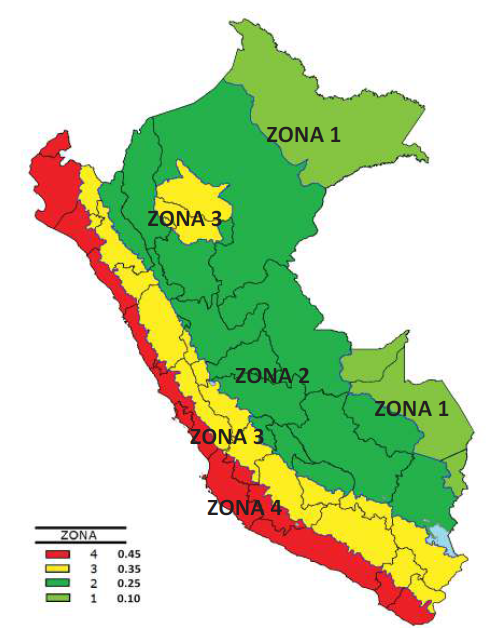
\includegraphics[width=4cm]{images/mapa_zona}%
\end{center}%
\end{minipage}%
\caption*{Fuente: E-30 (2018)}%
\end{table}

%
Las rigideces laterales pueden calcularse como la razon entre la fuerza cortante del entrepiso y el correspondiente desplazamiento relativo en el centro de masas, ambos evaluados para la misma condición de carga. \newline%
%
\subsection{Factor de suelo}%
\label{subsec:Factordesuelo}%
Las rigideces laterales pueden calcularse como la razon entre la fuerza cortante del entrepiso y el correspondiente desplazamiento relativo en el centro de masas, ambos evaluados para la misma condición de carga. \newline%
%


\begin{table}[ht!]%
\centering%
\caption{Factor de zona}%
\begin{tabular}{|>{\centering\arraybackslash}m{3.75cm}|>{\centering\arraybackslash}m{2cm}|>{\centering\arraybackslash}m{2cm}|>{\centering\arraybackslash}m{2cm}|>{\centering\arraybackslash}m{2cm}|}%
\hline%
\multicolumn{5}{|c|}{\textbf{FACTOR DE SUELO SEGÚN E{-}030}}\\%
\hline%
\backslashbox{\textit{\textbf{ZONA}}}{\textit{\textbf{SUELO}}}&\textbf{S0}&\textbf{S1}&\textbf{S2}&\textbf{S3}\\%
\hline%
4&0.80&1.00\cellcolor[rgb]{ .949,  .949,  .949} &1.05&1.10\\%
\hline%
3&0.80&1.00\cellcolor[rgb]{ .949,  .949,  .949} &1.15&1.20\\%
\hline%
2\cellcolor[rgb]{ .949,  .949,  .949} &0.80\cellcolor[rgb]{ .949,  .949,  .949} &\textcolor[rgb]{ 1,  0,  0}{\textbf{1.00}}\cellcolor[rgb]{ .949,  .949,  .949} \cellcolor[rgb]{ .949,  .949,  .949} &1.20\cellcolor[rgb]{ .949,  .949,  .949} &1.40\cellcolor[rgb]{ .949,  .949,  .949} \\%
\hline%
1&0.80&1.00\cellcolor[rgb]{ .949,  .949,  .949} &1.60&2.00\\%
\hline%
\end{tabular}%
\caption*{Fuente: E-30 (2018)}%
\end{table}

%
\subsubsection{Periodos de suelo}%
\label{ssubsec:Periodosdesuelo}%
%


\begin{table}[ht!]%
\centering%
\caption{Periodos de suelo}%
\begin{tabular}{|>{\centering\arraybackslash} m{2cm}|>{\centering\arraybackslash}m{2cm}|>{\centering\arraybackslash}m{2cm}|>{\centering\arraybackslash}m{2cm}|>{\centering\arraybackslash}m{2cm}|}%
\cline{2-5}%
\multicolumn{1}{r|}{}&\multicolumn{4}{c|}{\textbf{PERIODO "Tp" y "Tl" SEGÚN E-030}}\\%
\cline{2-5}%
\multicolumn{1}{r|}{}&\multicolumn{4}{c|}{\textit{\textbf{Perfil de suelo}}}\\%
\cline{2-5}%
\multicolumn{1}{r|}{}&\textbf{S0}&\textbf{S1}&\textbf{S2}&\textbf{S3}\\%
\hline%
Tp&0.30&\textcolor[rgb]{ 1,  0,  0}{\textbf{0.40}}\cellcolor[rgb]{ .949,  .949,  .949} &0.60&1.00\\%
\hline%
Tl&3.00&\textcolor[rgb]{ 1,  0,  0}{\textbf{2.50}}\cellcolor[rgb]{ .949,  .949,  .949} &2.00&1.60\\%
\hline%
\end{tabular}%
\caption*{Fuente: E-30 (2018)}%
\end{table}

%
Las rigideces laterales pueden calcularse como la razon entre la fuerza cortante del entrepiso y el correspondiente desplazamiento relativo en el centro de masas, ambos evaluados para la misma condición de carga. \newline%
%
\subsection{Sistema Estructural}%
\label{subsec:SistemaEstructural}%
Después de realizar el análisis sísmico se determino que los sistemas estructurales en X, Y son:%
Las rigideces laterales pueden calcularse como la razon entre la fuerza cortante del entrepiso y el correspondiente desplazamiento relativo en el centro de masas, ambos evaluados para la misma condición de carga. \newline%
%


\begin{table}[ht!]%
\caption{coeficiente básico de reducción}%
\begin{tabular}{|>{\arraybackslash}m{10cm}| >{\centering\arraybackslash}m{4cm}|}%
\hline%
\multicolumn{2}{|c|}{\textbf{SISTEMAS ESTRUCTURALES}}\\%
\hline%
\textbf{Sistema Estructural}&\multicolumn{1}{m{4cm}|}{\textbf{Coeficiente Básico de Reducción Ro}}\\%
\hline%
\multicolumn{2}{|l|}{\textbf{Acero:}}\\%
\hline%
Porticos Especiales Resistentes a Momento (SMF)&8\\%
\hline%
Porticos Intermedios Resistentes a Momento (IMF)&5\\%
\hline%
Porticos Ordinarios Resistentes a Momento (OMF)&4\\%
\hline%
Porticos Ordinarios Resistentes a Momento (OMF)&7\\%
\hline%
Porticos Ordinarios Concentricamente Arrriostrados (OCBF)&4\\%
\hline%
Porticos Excentricamente Arriostrados (EBF)&8\\%
\hline%
\multicolumn{2}{|l|}{\textbf{Concreto Armado:}}\\%
\hline%
Porticos&8\\%
\hline%
Dual&7\\%
\hline%
De muros estructurales&6\\%
\hline%
Muros de ductilidad limitada&4\\%
\hline%
\textbf{Albañilería Armada o Confinada}&3\\%
\hline%
\textbf{Madera}&7\\%
\hline%
\end{tabular}%
\caption*{Fuente: E-30 (2018)}%
\end{table}

%
\subsection{Factor de Amplificación sísmica}%
\label{subsec:FactordeAmplificacinssmica}%
Las rigideces laterales pueden calcularse como la razon entre la fuerza cortante del entrepiso y el correspondiente desplazamiento relativo en el centro de masas, ambos evaluados para la misma condición de carga. \newline%
%
Se determina según el artículo 11 de la E{-}30%
\setlength{\jot}{0.5cm}%


\begin{figure}[h!]%
\caption{Factor de amplificación}%
\begin{minipage}{0.5\textwidth}%

    \begin{align*}
        &T< T_{P}         &   C&=2,5\cdot\left ( \frac{T_{P}}{T} \right )\\
        &T_{P}< T< T_{L}  &   C&=2,5\cdot\left ( \frac{T_{P}}{T} \right )\\
        &T> T_{L}         &   C&=2,5\cdot\left ( \frac{T_{P}\;T_{L}}{T^{2}} \right )
    \end{align*}%
\end{minipage}%
\begin{minipage}{0.4\textwidth}%
\centering%
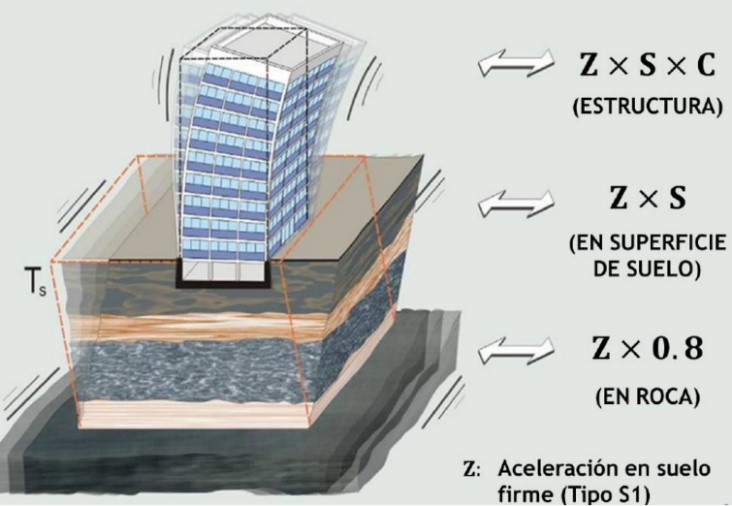
\includegraphics[width=6.5cm]{images/Amplificacion}%
\end{minipage}%
\caption*{Fuente: Muñoz (2020)}%
\end{figure}

%
\subsubsection{Factor de Importancia}%
\label{ssubsec:FactordeImportancia}%
%


\begin{table}[h!]%
\centering%
\caption{Factor de Uso o Importancia}%
\begin{tabular}{|>{\arraybackslash}m{3cm}|m{8cm}|>{\arraybackslash}m{2.8cm}|}%
\hline%
\multicolumn{3}{|c|}{\textbf{CATEGORIA DE LA EDIFICACION}}\\%
\hline%
\multicolumn{1}{|c|}{\textbf{CATEGORIA}}&\multicolumn{1}{|c|}{\textbf{DESCRIPCION}}&\multicolumn{1}{|c|}{\textbf{FACTOR U}}\\%
\hline%
\multirow{2}[4]{3cm}{A Edificaciones Escenciales}&A1: Establecimiento del sector salud (públicos y privados) del segundo y tercer nivel, según lo normado por el ministerio de salud.&\multicolumn{1}{>{\centering\arraybackslash}m{2.8cm}|}{Con aislamiento 1.0 y sin aislamiento 1.5.}\\%
\cline{2-3}%
&A2: Edificaciones escenciales para el manejo de las emergencias, el funcionamiento del gobierno y en general aquellas que puedan servir de refugio después de un desastre.\cellcolor[rgb]{1,  .949,  .8}&\multicolumn{1}{>{\centering\arraybackslash}m{2.8cm}|}{\textcolor[rgb]{ 1,  0,  0}{\textbf{1.50}}\cellcolor[rgb]{1,  .949,  .8}}\\%
\hline%
B Edificaciones Importantes &Edificaciones donde se reúnen gran cantidad de personas tales como cines, teatros, estadios, coliseos, centros comerciales, terminales de buses de pasajeros, establecimientos penitenciarios, o que guardan patrimonios valiosos como museos y bibliotecas.&\multicolumn{1}{>{\centering\arraybackslash}m{2.8cm}|}{1.30}\\%
\hline%
C Edificaciones Comunes&Edificaciones comunes tales como: viviendas, oficinas, hoteles, restaurantes, depósitos e instalaciones industriales cuya falla no acarree peligros adicionales de incendios o fugas de contaminantes.&\multicolumn{1}{>{\centering\arraybackslash}m{2.8cm}|}{1.00}\\%
\hline%
D Edificaciones temporales&Construcciones provisionales para depósitos, casetas y otras similares.&\multicolumn{1}{>{\centering\arraybackslash}m{2.8cm}|}{A criterio del proyectista}\\%
\hline%
\end{tabular}%
\caption*{Fuente: E-30 (2018)}%
\end{table}

%
\subsubsection{Análisis modal Art. 26.1 E{-}030}%
\label{ssubsec:AnlisismodalArt.26.1E{-}030}%
\begin{tcolorbox}[colback=gray!5!white,colframe=Maroon!75!black,fonttitle=\bfseries,title=Art. 26.1.1]%
\textit{En cada dirección se consideran aquellos modos de vibración cuya suma de masas efectivas sea por lo menos el 90\% de la masa total, pero se toma en cuenta por lo menos los tres primeros modos predominantes en la dirección de análisis.}%
\end{tcolorbox}%
\begin{tcolorbox}[colback=gray!5!white,colframe=Maroon!75!black,fonttitle=\bfseries,title=Art. 26.1.2]%
\textit{En cada dirección se consideran aquellos modos de vibración cuya suma de masas efectivas sea por lo menos el 90\% de la masa total, pero se toma en cuenta por lo menos los tres primeros modos predominantes en la dirección de análisis.}%
\end{tcolorbox}%
Las rigideces laterales pueden calcularse como la razon entre la fuerza cortante del entrepiso y el correspondiente desplazamiento relativo en el centro de masas, ambos evaluados para la misma condición de carga. \newline%
%


\begin{table}[h!]%
\extrarowheight = -0.3ex%
\renewcommand{\arraystretch}{1.3}%
\centering%
\caption{Periodos y porcentajes de masa participativa}%
\begin{tabular}{cccccccc}
\toprule
Mode & Period & UX & UY & RZ & SumUX & SumUY & SumRZ \\
\midrule
1 & 0.644 & 0.691 & 0.001 & 0.011 & 0.691 & 0.001 & 0.011 \\
2 & 0.451 & 0.016 & 0.017 & 0.663 & 0.706 & 0.018 & 0.675 \\
3 & 0.218 & 0.000 & 0.654 & 0.018 & 0.707 & 0.672 & 0.693 \\
4 & 0.176 & 0.131 & 0.001 & 0.002 & 0.838 & 0.672 & 0.695 \\
5 & 0.130 & 0.001 & 0.001 & 0.017 & 0.839 & 0.674 & 0.712 \\
6 & 0.122 & 0.002 & 0.001 & 0.100 & 0.841 & 0.675 & 0.812 \\
7 & 0.100 & 0.000 & 0.003 & 0.030 & 0.841 & 0.678 & 0.842 \\
8 & 0.087 & 0.019 & 0.000 & 0.007 & 0.861 & 0.678 & 0.848 \\
9 & 0.076 & 0.034 & 0.000 & 0.000 & 0.894 & 0.678 & 0.848 \\
10 & 0.064 & 0.001 & 0.000 & 0.002 & 0.895 & 0.678 & 0.850 \\
11 & 0.054 & 0.000 & 0.001 & 0.049 & 0.896 & 0.678 & 0.899 \\
12 & 0.050 & 0.001 & 0.056 & 0.001 & 0.897 & 0.735 & 0.900 \\
13 & 0.050 & 0.001 & 0.123 & 0.001 & 0.898 & 0.858 & 0.901 \\
14 & 0.049 & 0.007 & 0.000 & 0.000 & 0.905 & 0.858 & 0.901 \\
15 & 0.046 & 0.019 & 0.000 & 0.002 & 0.924 & 0.858 & 0.903 \\
16 & 0.042 & 0.000 & 0.000 & 0.000 & 0.924 & 0.858 & 0.903 \\
17 & 0.037 & 0.000 & 0.000 & 0.000 & 0.924 & 0.858 & 0.903 \\
18 & 0.035 & 0.001 & 0.000 & 0.020 & 0.925 & 0.858 & 0.924 \\
19 & 0.034 & 0.001 & 0.000 & 0.002 & 0.925 & 0.858 & 0.926 \\
20 & 0.033 & 0.006 & 0.000 & 0.001 & 0.931 & 0.858 & 0.927 \\
21 & 0.032 & 0.004 & 0.000 & 0.000 & 0.935 & 0.858 & 0.927 \\
22 & 0.031 & 0.006 & 0.000 & 0.002 & 0.941 & 0.858 & 0.929 \\
23 & 0.026 & 0.004 & 0.000 & 0.008 & 0.945 & 0.858 & 0.937 \\
24 & 0.024 & 0.006 & 0.000 & 0.000 & 0.951 & 0.858 & 0.937 \\
\bottomrule
\end{tabular}
%
\end{table}

%
\subsubsection{Irregularidad de Rigidez{-}Piso Blando}%
\label{ssubsec:IrregularidaddeRigidez{-}PisoBlando}%
\begin{tcolorbox}[colback=gray!5!white,colframe=cyan!75!black,fonttitle=\bfseries,title=Tabla N°9 E-030]%
Existe irregularidad de rigidez cuando, en cualquiera de las direcciondes de análisis, en un entrepiso la rigidez lateral es menor que 70\% de la rigidez lateral del entrepiso inmediato superior, o es menor que 80\% de la rigidez lateral promedio de los tres niveles superiores adyacentes. 
 Las rigideces laterales pueden calcularse como la razón entre la fuerza cortante del entrepiso y el correspondiente desplazamiento relatibo en el centro de masas, ambos evaluados para la misma condición de carga %
\end{tcolorbox}%
\begin{tcolorbox}[colback=gray!5!white,colframe=cyan!75!black,fonttitle=\bfseries,title=Tabla N°9 E-030]%

Existe irregularidad extrema de rigidez cuando, en cualquiera de las direcciones de análisis, en un entrepiso la rigidez lateral es menor que 60\% de la rigidez lateral del entrepiso inmediato superior, o es menor que 70\% de la rigidez lateral promedio de los tres niveles superiores adyacentes.
Las rigideces laterales pueden calcularse como la razon entre la fuerza cortante del entrepiso y el correspondiente desplazamiento relativo en el centro de masas, ambos evaluados para la misma condición de carga.%
\end{tcolorbox}%
Las rigideces laterales pueden calcularse como la razon entre la fuerza cortante del entrepiso y el correspondiente desplazamiento relativo en el centro de masas, ambos evaluados para la misma condición de carga. \newline%
%


\begin{table}[h!]%
\centering%
\caption{Irregularidad de rigidez}%
\begin{tabular}{cccccccc}
\toprule
Story & OutputCase & VX & VY & Rigidez Lateral(k) & 70\%k previo & 80\%Prom(k) & is\_reg \\
\midrule
Story8 & SDx Max & 16.998 & 0.844 & 7535.714 &  &  & Regular \\
Story7 & SDx Max & 34.801 & 1.727 & 15987.963 & 5275.000 &  & Regular \\
Story6 & SDx Max & 49.265 & 2.437 & 19039.063 & 11191.574 &  & Regular \\
Story5 & SDx Max & 60.929 & 3.010 & 21194.366 & 13327.344 & 11350.064 & Regular \\
Story4 & SDx Max & 70.491 & 3.478 & 24846.429 & 14836.056 & 14992.371 & Regular \\
Story3 & SDx Max & 77.406 & 3.810 & 29997.638 & 17392.500 & 17354.629 & Regular \\
Story2 & SDx Max & 81.495 & 3.992 & 40326.263 & 20998.346 & 20276.915 & Regular \\
Story1 & SDx Max & 82.631 & 4.029 & 175195.652 & 28228.384 & 25378.754 & Regular \\
\bottomrule
\end{tabular}
%
\end{table}

%


\begin{table}[h!]%
\centering%
\caption{Irregularidad de rigidez}%
\begin{tabular}{cccccccc}
\toprule
Story & OutputCase & VX & VY & Rigidez Lateral(k) & 70\%k previo & 80\%Prom(k) & is\_reg \\
\midrule
Story8 & SDy Max & 0.953 & 19.257 & 40885.350 &  &  & Regular \\
Story7 & SDy Max & 1.804 & 39.310 & 79414.949 & 28619.745 &  & Regular \\
Story6 & SDy Max & 2.451 & 54.588 & 108958.283 & 55590.465 &  & Regular \\
Story5 & SDy Max & 2.973 & 66.249 & 135201.224 & 76270.798 & 61135.622 & Regular \\
Story4 & SDy Max & 3.465 & 75.805 & 166238.816 & 94640.857 & 86286.522 & Regular \\
Story3 & SDy Max & 3.878 & 83.019 & 210709.137 & 116367.171 & 109439.553 & Regular \\
Story2 & SDy Max & 4.154 & 87.479 & 295538.176 & 147496.396 & 136573.114 & Regular \\
Story1 & SDy Max & 4.230 & 88.650 & 757692.308 & 206876.723 & 179329.634 & Regular \\
\bottomrule
\end{tabular}
%
\end{table}

%
\subsection{Irregularidad de Masa o Peso}%
\label{subsec:IrregularidaddeMasaoPeso}%
\begin{tcolorbox}[colback=gray!5!white,colframe=cyan!75!black,fonttitle=\bfseries,title=Tabla N°9 E-030]%
Se tiene irregularidad de masa (o peso) cuando el peso de un piso determinado según el artículo 26, es nayor que 1,5 veces el peso de un piso adyascente. Este criterio no se aplica en azoteas ni en sótanos%
\end{tcolorbox}%
Las rigideces laterales pueden calcularse como la razon entre la fuerza cortante del entrepiso y el correspondiente desplazamiento relativo en el centro de masas, ambos evaluados para la misma condición de carga. \newline%
%


\begin{table}[h!]%
\centering%
\caption{Irregularidad de Masa o Peso}%
\begin{tabular}{ccccc}
\toprule
Story & Masa & 1.5 Masa & Tipo de Piso & is\_reg \\
\midrule
Story8 & 6.669 &  & Azotea & Regular \\
Story7 & 8.754 & 13.130 & Piso & Regular \\
Story6 & 8.737 & 13.106 & Piso & Regular \\
Story5 & 8.739 & 13.109 & Piso & Regular \\
Story4 & 9.163 & 13.745 & Piso & Regular \\
Story3 & 9.163 & 13.745 & Piso & Regular \\
Story2 & 9.163 & 13.745 & Piso & Regular \\
Story1 & 7.434 & 11.150 & Piso & Irregular \\
NT & 3.560 & 5.340 & Piso & Regular \\
Base & 3.918 &  & Sotano & Regular \\
\bottomrule
\end{tabular}
%
\end{table}

%
\newpage%
\subsubsection{Irregularidad Torsional}%
\label{ssubsec:IrregularidadTorsional}%
\begin{tcolorbox}[colback=gray!5!white,colframe=cyan!75!black,fonttitle=\bfseries,title=Tabla N°9 E-030]%
Existe irregularidad torsional cuando, en cualquiera de las direcciones de análisis el desplazamiento relativo de entrepiso en un edificion ($\Delta_{max}$) en esa dirección, calculado incluyendo excentricidad accidental, es mayor que 1,3 veces el desplazamineto relativo promedio de los extremos del mismo entrepiso para la condicion de carga ($\Delta_{prom}$). 
 Este crriterio sólo se aplica en edificios con diafragmas rígidos y sólo si el máximo desplazamiento relativo de entrepiso es mayor que 50\% del desplazamiento permisible indicado en la Tabla N° 11%
\end{tcolorbox}%
\begin{tcolorbox}[colback=gray!5!white,colframe=cyan!75!black,fonttitle=\bfseries,title=Tabla N°9 E-030]%
Existe irregularidad torsional cuando, en cualquiera de las direcciones de análisis el desplazamiento relativo de entrepiso en un edificion ($\Delta_{max}$) en esa dirección, calculado incluyendo excentricidad accidental, es mayor que 1,3 veces el desplazamineto relativo promedio de los extremos del mismo entrepiso para la condicion de carga ($\Delta_{prom}$). 
 Este crriterio sólo se aplica en edificios con diafragmas rígidos y sólo si el máximo desplazamiento relativo de entrepiso es mayor que 50\% del desplazamiento permisible indicado en la Tabla N° 11%
\end{tcolorbox}%
%


\begin{table}[ht!]%
\centering%
\caption{Irregularidad Torsional}%
\resizebox{\textwidth}{!}{%
\begin{tabular}{cccccccccc}
\toprule
Story & OutputCase & Direction & Max Drift & Avg Drift & Ratio & Height & Drifts & < Driftmax/2 & Es Regular \\
\midrule
Story8 & SDx Max & X & 0.003021 & 0.002475 & 1.221 & 2.5 & 0.007250 & False & Regular \\
Story7 & SDx Max & X & 0.003476 & 0.002869 & 1.211 & 2.5 & 0.008342 & False & Regular \\
Story6 & SDx Max & X & 0.004116 & 0.003335 & 1.234 & 2.5 & 0.009878 & False & Regular \\
Story5 & SDx Max & X & 0.00454 & 0.003673 & 1.236 & 2.5 & 0.010896 & False & Regular \\
Story4 & SDx Max & X & 0.004657 & 0.003773 & 1.234 & 2.5 & 0.011177 & False & Regular \\
Story3 & SDx Max & X & 0.004479 & 0.003582 & 1.25 & 2.5 & 0.010750 & False & Regular \\
Story2 & SDx Max & X & 0.003811 & 0.002958 & 1.288 & 2.5 & 0.009146 & False & Regular \\
Story1 & SDx Max & X & 0.001124 & 0.000904 & 1.244 & 1.5 & 0.004496 & False & Regular \\
NT & SDx Max & X & 0.00024 & 0.00012 & 2 & 1.75 & 0.000823 & True & Regular \\
NT & SDx Max & Y & 2.8E-05 & 1.4E-05 & 2 & 1.75 & 0.000096 & True & Regular \\
\bottomrule
\end{tabular}
}%
\end{table}

%


\begin{table}[ht!]%
\centering%
\caption{Irregularidad Torsional}%
\resizebox{\textwidth}{!}{%
\begin{tabular}{cccccccccc}
\toprule
Story & OutputCase & Direction & Max Drift & Avg Drift & Ratio & Height & Drifts & < Driftmax/2 & Es Regular \\
\midrule
Story8 & SDy Max & X & 0.000535 & 0.000322 & 1.662 & 2.5 & 0.001284 & True & Regular \\
Story8 & SDy Max & Y & 0.000498 & 0.000478 & 1.042 & 2.5 & 0.001195 & True & Regular \\
Story7 & SDy Max & X & 0.00059 & 0.000357 & 1.65 & 2.5 & 0.001416 & True & Regular \\
Story7 & SDy Max & Y & 0.000527 & 0.00051 & 1.033 & 2.5 & 0.001265 & True & Regular \\
Story6 & SDy Max & X & 0.000632 & 0.000387 & 1.633 & 2.5 & 0.001517 & True & Regular \\
Story6 & SDy Max & Y & 0.000533 & 0.000517 & 1.031 & 2.5 & 0.001279 & True & Regular \\
Story5 & SDy Max & X & 0.00065 & 0.000402 & 1.618 & 2.5 & 0.001560 & True & Regular \\
Story5 & SDy Max & Y & 0.000523 & 0.000506 & 1.034 & 2.5 & 0.001255 & True & Regular \\
Story4 & SDy Max & X & 0.000637 & 0.000397 & 1.605 & 2.5 & 0.001529 & True & Regular \\
Story4 & SDy Max & Y & 0.000488 & 0.000471 & 1.035 & 2.5 & 0.001171 & True & Regular \\
Story3 & SDy Max & X & 0.000577 & 0.000361 & 1.597 & 2.5 & 0.001385 & True & Regular \\
Story3 & SDy Max & Y & 0.000423 & 0.000407 & 1.038 & 2.5 & 0.001015 & True & Regular \\
Story2 & SDy Max & X & 0.00046 & 0.000287 & 1.602 & 2.5 & 0.001104 & True & Regular \\
Story2 & SDy Max & Y & 0.000332 & 0.000313 & 1.058 & 2.5 & 0.000797 & True & Regular \\
Story1 & SDy Max & X & 0.000167 & 0.000103 & 1.625 & 1.5 & 0.000668 & True & Regular \\
Story1 & SDy Max & Y & 0.000126 & 0.000108 & 1.173 & 1.5 & 0.000504 & True & Regular \\
NT & SDy Max & X & 3.3E-05 & 1.6E-05 & 2 & 1.75 & 0.000113 & True & Regular \\
NT & SDy Max & Y & 2.7E-05 & 1.3E-05 & 2 & 1.75 & 0.000093 & True & Regular \\
\bottomrule
\end{tabular}
}%
\end{table}

%
\subsubsection{Irregularidad por Esquinas Entrantes}%
\label{ssubsec:IrregularidadporEsquinasEntrantes}%
\begin{tcolorbox}[colback=gray!5!white,colframe=cyan!75!black,fonttitle=\bfseries,title=Tabla N°9 E-030]%
\textit{La estructura se califica como irregular cuando los diafragmas tienen discontinuidades abruptas o variaciones importantes en rigidez, incluyendo aberturas mayores que 50\% del área bruta del diafragma.} \\ \textit{También  existe  irregularidad  cuando,  en  cualquiera de  los pisos y para cualquiera de las direcciones de análisis, se tiene alguna sección transversal del diafragma con un área neta resistente menor que 25\% del área de la sección transversal total de la misma dirección calculada con las dimensiones totales de la planta.}%
\end{tcolorbox}%


\begin{figure}[ht!]%
\centering%
\caption{Irregularidad por discontinuidad del diafragma}%
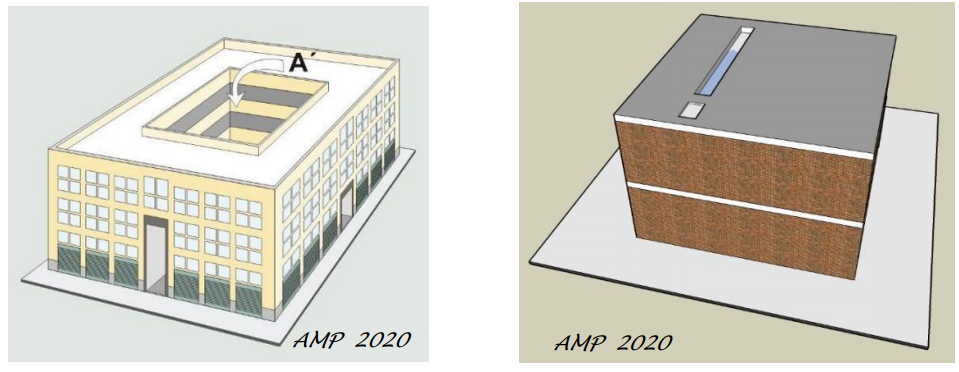
\includegraphics[scale=0.7]{images/i_diafragma.PNG}%
\caption*{\small Fuente: Muñoz (2020)}%
\end{figure}

%


\begin{table}[H]%
\centering%
\caption{Irregularidad por discontinuidad del diafragma (a)}%
\begin{tabular}{|ll|c|r}%
\cline{1-3}%
\multicolumn{2}{|l|}{Longitud del aligerado (L1)} & 7.51 & \multicolumn{1}{l}{m} \\%
\cline{1-3}%
\multicolumn{2}{|l|}{Espesor del aligerado (e1)} & 0.05 & \multicolumn{1}{l}{m} \\%
\cline{1-3}%
\multicolumn{2}{|l|}{Area del aligerado A1=L1$\cdot$ e1} & 0.38 & \multicolumn{1}{l}{$m^2$} \\%
\cline{1-3}%
\multicolumn{2}{|l|}{Longitud de la losa macisa (L2)} & 2.25 & \multicolumn{1}{l}{m} \\%
\cline{1-3}%
\multicolumn{2}{|l|}{Espesor de la losa macisa (e2)} & 0.2 & \multicolumn{1}{l}{m} \\%
\cline{1-3}%
\multicolumn{2}{|l|}{Area de la losa macisa A1=L1$\cdot$ e1} & 0.45 & \multicolumn{1}{l}{$m^2$} \\%
\cline{1-3}%
\multicolumn{2}{|l|}{Ratio} & 118.42 & \multicolumn{1}{l}{\%} \\%
\cline{1-3}%
\multicolumn{2}{|l|}{Ratio límite} & 25.00 & \multicolumn{1}{l}{\%} \\%
\cline{1-3}%
\multicolumn{2}{|l|}{Verificación} & \textcolor[rgb]{ .267,  .447,  .769}{\textbf{Regular}} & \multicolumn{1}{l}{} \\%
\cline{1-3}%
\end{tabular}%
\end{table}

%


\begin{table}[H]%
\centering%
\caption{Irregularidad por discontinuidad del diafragma (b)}%
\begin{tabular}{cccc}%
\hline%
\textbf{Abertura}&\textbf{Largo (m)}&\textbf{Ancho (m)}&\textbf{Área $m^2$}\\%
\hline%
1&4.02&2.30&9.25\\%
\hline%
2&1.10&2.30&2.53\\%
\hline%
3&1.20&19.00&22.80\\%
\hline%
&\multicolumn{2}{r}{Área total de aberturas:}&34.58 $m^2$\\%
&\multicolumn{2}{r}{Área total de la planta:}&120.41 $m^2$\\%
&\multicolumn{2}{r}{Ratio:}&28.72 \%\\%
&\multicolumn{2}{r}{Ratio límite:}&50.00 \%\\%
&\multicolumn{2}{r}{Verificación:}&\textcolor[rgb]{ .267,  .447,  .769} {Regular}\\%
\end{tabular}%
\end{table}

%
Las rigideces laterales pueden calcularse como la razon entre la fuerza cortante del entrepiso y el correspondiente desplazamiento relativo en el centro de masas, ambos evaluados para la misma condición de carga. \newline%
%
\end{document}